\section{Fallbeispiel AXA Gesundheitsvorsorge}

In diesem Kapitel wird die Anwendbarkeit der künstlichen Intelligenz zur automatisierten Verarbeitung von eingereichten Rechnungen bei der AXA Gesundheitsvorsorge überprüft.

Es wird erst ein Überblick über den Prozess gewährt, aus welchem anschliessend Aufgaben abgeleitet werden, welche mit Hilfe von künstlicher Intelligenz automatisiert werden sollen.

\subsection{Einleitung}

\todo[inline]{Grober Abriss über den Umfang des Prototypen

Umfang reduzieren auf 2 Teilaspekte:

- Rechnungsklassifizierung (hierzu 2 Ansätze (Pixel vs. OCR) vergleichen)

- Informationsextraktion (e.g. von Patienten namen und des Totalbetrags)
}

Der Prozess der Rechnungseinreichung und -verarbeitung (vgl. Abbildung \ref{prozessaxa}) der AXA kann aufgrund zwei verschiedener Ereignisse angestossen werden. In jedem Fall reicht der Kunde eine Rechnung ein. Dies kann er entweder digital, im Kundenportal, oder per Post machen. 

\begin{figure}[h]
    \captionsetup{width=.8\linewidth}
    \caption{Prozess der Rechnungseinreichung und -verarbeitung der AXA Gesundheitsvorsorge. Vom Kunden per Post oder über das Kundenportal eingereichte Rechnungen durchlaufen mehrere Prozessschritte in Verantwortung unterschiedlicher Organisationen.}
    \label{prozessaxa}
    \centering
    \vspace{0.2cm}
    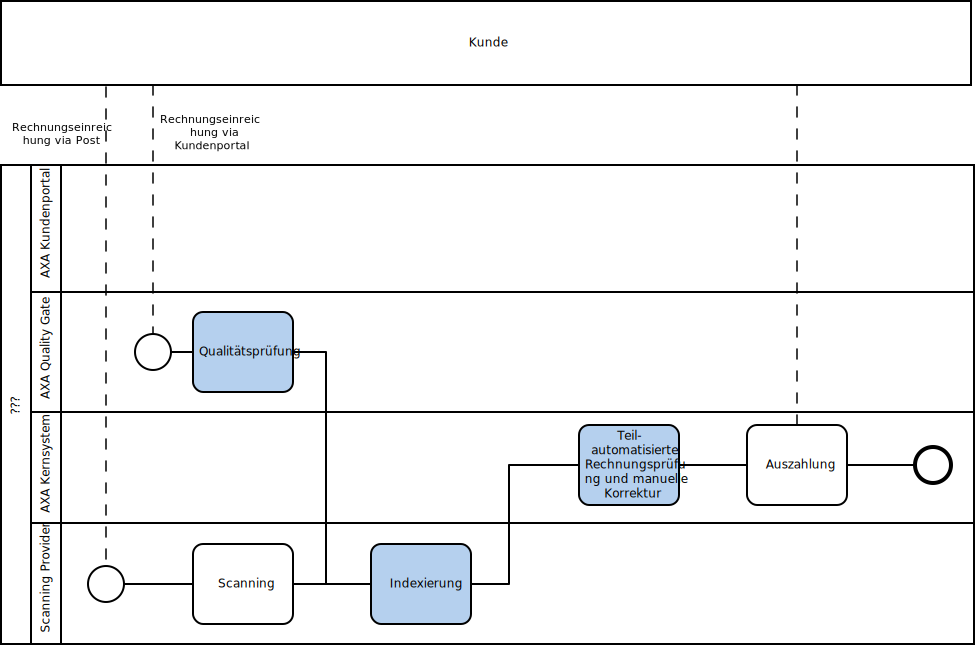
\includegraphics[width=\textwidth]{graphics/rechnungseinreichung-bpmn.pdf}
\end{figure}

\todo[inline]{Im BPMN Diagramm SVG export fehlen die Pfeile...}

Im Kundenportal hat der Kunde die Möglichkeit eine Rechnung hochzuladen. Dabei kann er entweder ein Dokument auf seinem Endgerät wählen oder die Kamera seines Geräts nutzen, um eine Rechnung zu fotografieren.

Nach erfolgreichem Hochladen der Rechnung im Kundenportal durchläuft diese eine erste manuelle Qualitätsprüfung. Diese Qualitätsprüfung wurde eingeführt, da hochgeladene Rechnung teilweise ungenügende Qualität vorweisen. Entspricht die Rechnung nicht den Qualitätsanforderungen oder fehlt eine Seite oder eine ärztliche Verordnung, so wird der Kunde gebeten, die vollständige Rechnung erneut hochzuladen.

Nach erfolgreicher Qualitätsprüfung wird die Rechnung an den Scanning und Indexierungsdienstleister der AXA weitergeleitet.

Entscheidet sich der Kunde für die Einreichung per Post, so wird sein Brief direkt an den Scanning und Indexierungsdienstleister der AXA weitergeleitet, bei welchem die Rechnung eingescannt wird.

Nach beiden dieser Einstiegspunkten in den Prozess indexiert nun der Scanning und Indexierungsdienstleister der AXA die eingereichte Rechnung. Dieser Aufgabenschritt erfolgt teilweise automatisiert und teilweise manuell. Wie genau die Indexierung abläuft ist nicht bekannt, da diese Dienstleistung eingekauft wird.

Nach der Indexierung werden die Scans sowie das strukturierte Resultat der Indexierung elektronisch an das Kernsystem der AXA Gesundheitsvorsorge übermittelt. Dieses Kern\-system verarbeitet die eingegangenen Rechnungen aufgrund eines Regelwerks. Kann die Rechnung nicht verarbeitet werden, weil diese nicht korrekt Indexiert wurde oder Informationen fehlen, muss eine FachspezialistIn eingreiffen. Nach allfälligen Rückfragen und Korrekturen durch die FachspezialistIn wird die Rechnung verarbeitet. 

Nach der Erfolgreichen Verarbeitung der Rechnung wird der Kunde elektronisch informiert, ob die beanspruchten Leistungen versichert sind und ob eine Rückvergütung ausbezahlt wird.

Hat der Kunde die AXA bevollmächtigt, so wird die Rechnung in gewissen Fällen, je nach Rechnungspositionen, automatisiert an die Grundversicherung des Kunden weitergeleitet. 

Ziel der AXA Gesundheitsvorsorge ist es, diesen Prozess für eingereichte Rechnungen, welche Fitnesscenter und Optiker betreffen, vollständig zu automatisieren. Dabei gibt es in diversen Bereichen Herausforderungen, welche aktuell angegangen werden. Diese Arbeit hat zum Ziel, die Herausforderungen im Bereich der Indexierung anzugehen. Es wird untersucht, ob die Anwendung künstlicher Intelligenz eine Automatisierung der Indexierung ermöglichen kann.

% Um den Umfang dieser Analyse einzugrenzen, wird der Fokus auf Rechnungen von Optikern, Fitnesscentern und Sportvereinen gelegt. Diese Rechnungen machen 23\% der eingereichten Rechnungen aus und sind Versicherungstechnisch relativ einfach handzuhaben.

% optiker 2660 -> 
% fitness 2055
% sportsclub 847
% =subtotla 5562
% other 18881
% =total 24443


\subsection{Vorgehen und Methodik}

\todo[inline]{Abschnitt überarbeiten...}

Die Anwendbarkeit der künstlichen Intelligenz für dieses Fallbeispiel wird durch zwei praktische Experimente geprüft. Dafür werden zuerst die Anforderungen und Bewertungskriterien an die Indexierung gesammelt und anschliessend Teilaufgaben abgeleitet. 

Für jede Teilaufgabe werden Messkriterien definiert, welche die Grundlagen für die Bewertung der Gesamtaufgabe bilden. Es wird für jede Teilaufgabe mindestens ein Experiment durchgeführt.

Für jedes Experiment wird eine aufgabenspezifische künstliche Intelligenz geschaffen, welche anhand der für die Teilaufgabe definierten Messkriterien bewertet wird.

\subsection{Anforderungen}

Um Rechnungen von Fitnesscenter und Optikern automatisiert verarbeiten zu können, müssen diese Rechnungen erkannt und die notwendigen Informationen, welche nachfolgend genauer spezifiziert werden, extrahiert werden.

Um eine Rechnung eines Optikers zu verarbeiten, sind folgende Informationen relevant:

\begin{itemize}
    \item \textbf{Leistungsbezüger}
    
    Es muss ermittelt werden, für wen die Rechnung ausgestellt wurde. Anhand dieser Information wird geprüft, ob und wie diese Person bei der AXA versichert ist. Auch wird damit geprüft, dass der maximal versicherte Betrag noch nicht ausgeschöpft ist.
    
    Ist der Leistungsbezüger minderjährig, so wird ein gewisser Betrag von der Grundversicherung übernommen. In diesem Fall wird dieser Betrag von der Rückvergütung der AXA abgezogen und die Rechnung an die Grundversicherung weitergeleitet.
    
    \item \textbf{Totalbetrag der Rechnung (inkl. Währung)}
    
    Dieser Betrag bildet die Grundlage zur Berechnung der geschuldeten Leistung an den Kunden. 
    
    Einzelne Rechnungspositionen sind für Rechnungen von Optikern nicht relevant.
    
    \item \textbf{Hinweis auf eine ärztliche Verordnung}
    
    Besteht eine ärztliche Verordnung, ist ein gewisser Betrag bei der Grundversicherung versichert. In diesem Fall wird dieser Betrag von der Rückvergütung der AXA abgezogen und die Rechnung an die Grundversicherung weitergeleitet.
\end{itemize}

%\paragraph{
%    \textbf{Relevante Attribute einer Rechnung für einen Sportverein}
%}

%Eine Rechnung eines Sportvereins wird bei der AXA Anhand folgender Attribute beurteilt:

%\begin{itemize}
%    \item \textbf{Leistungsbezüger}
%    
%    Es muss ermittelt werden, für wen die Rechnung ausgestellt wurde. Anhand dieser Information wird geprüft ob und wie diese Person bei der AXA Versichert ist. Auch wird damit geprüft, dass der maximal versicherte Betrag noch nicht ausgeschöpft ist.
%    \item \textbf{Totalbetrag der Rechnung (inkl. Währung):}
%    
%    Dieser Betrag bildet die Grundlage zur Berechung des geschuldeten Betrages. 
%    
%    Einzelne Rechnungspoisition sind für Rechnungen eines Sportvereins nicht relevant.
%    \item \textbf{Sportart}
%    
%    Die AXA anerkennt alle olympischen Sportarten. Das bedeutet, gewisse Sportarten sind nicht versichert. Es muss also die Sportart ermittelt werden, um die Versicherungsdeckung zu prüfen.
%\end{itemize}

Folgende Informationen sind relevant, um eine Rechnung für ein Fitness-Abo zu verarbeiten:

\begin{itemize}
    \item \textbf{Leistungsbezüger}
    
    Es muss ermittelt werden, für wen die Rechnung ausgestellt wurde. Anhand dieser Information wird geprüft ob und wie diese Person bei der AXA versichert ist. Auch wird damit geprüft, dass der maximal versicherte Betrag noch nicht ausgeschöpft ist.
    \item \textbf{Totalbetrag der Rechnung (inkl. Währung):}
    
    Dieser Betrag bildet die Grundlage zur Berechnung der geschuldeten Leistung an den Kunden. 
    
    Einzelne Rechnungspositionen sind für Rechnungen von Optikern nicht relevant.
    \item \textbf{Fitnesscenter (Leistungserbringer)}
    
    Die AXA anerkennt alle Fitnesscenter mit dem Label Qualitop von Qualicert oder mit einer Bewertung von mindestens 3 Sternen bei Fitnessguide.
\end{itemize}

Anahnd dieser Informationen können Rechnungen automatisiert verarbeitet werden. Es ist wichtig, dass diese Informationen korrekt extrahiert werden. Durch die Automatisierung entfällt jegliche manuelle Prüfung und Fehler würden, wenn überhaupt, erst dem Kunden auffallen. 

\todo[inline]{Hier definieren:

- Wieviel \% der Fitness und Optiker Rechnungen sollen automatisiert verarbeitet werden

- Wie viele Fehler dürfen gemacht werden (Falsche klassifiziert, falsche Beträge, falsche Leistungsbezüger)

- ... andere Metriken}

\subsection{Übersicht}

\todo[inline]{Überarbeiten}

Um die Aufgabenstellung besser zu verstehen und Schrittweise bearbeiten zu können, wird diese in zwei Teilaufgaben unterteilt. 

Im ersten Schritt werden Rechnungen klassifiziert, damit Rechnungen von Optikern und Fitnesscentern zur weiteren Verarbeitung ausgelenkt werden können. 

Im zweiten Schritt werden die notwendigen Informationen aus den Rechnungen extrahiert. Die Klassifizierung aus dem ersten Schritt erlaubt es, in diesem Schritt ein System zu verwenden, welches auf eine Klasse von Rechnungen spezialisiert ist. 

\subsection{Teil 1 - Klassifizierung von Rechnungen}

Die Klassifizierung dient dazu, eine Rechnung einer bestimmten Art (Klasse) zuzuweisen. Die Klassen \enquote{Optiker} und \enquote{Fitness} sind durch die Anforderungen gegeben. Neben diesen Klassen könnten Rechnungen noch in viele weitere Klassen eingeteilt werden. Um dem Rechnung zu tragen, werden in diesem Experiment  Rechnungen den Klassen \enquote{Optiker}, \enquote{Fitness}, \enquote{Sportverein} und \enquote{Übrige} zugewiesen. In der späteren Anwendung wäre es denkbar, die Anzahl Klassen zu erhöhen und somit auch andere Arten von Rechnungen zu Automatisieren.

Als Ausgangspunkt für die Klassifizierung steht ein Bild einer Rechnung. Die Klassifizierung von Bildern respektive Fotos ist eine bekannte Problematik der Computer Vision und bildet in diesem Bereich die Grundlage für die Lösung vieler weiterer Problematiken~\autocite{StanfordGithubClassification}. 

% Die Wichtigkeit der Bildklassifizierung zeigt die Organisation ImageNet. ImageNet aht es zum Ziel, Forschern einen einfachen Zugang zu Datensätzen von Bildern zu gewähren. Seit 2010 wurden bereits sieben Wettbewerbe im Bereich der Computer Vision veranstaltet rund um die Klassifizierung von Bildern und die Erkennung von Objekten auf diesen Bildern~\autocite{ImageNet2019}. 

Es liegt nahe, die Klassifizierung der Rechnungen mit Bild-basierten Modellen aus dem Bereich der Computer Vision anzugehen. Im folgenden Kapitel wird dieser Ansatz verfolgt.

Nicht nur im Bereich der Computer Vision ist die Problematik der Klassifizierung ein viel behandeltes Themengebiet. Im Bereich des Natural Language Processing ist die Klassifizierung von Wörtern, Sätzen oder ganzen Texten eine bekannte Problemstellung. Die sogenannte Text Classification ist die Grundlage für viele Applikationen, welche mit Texten arbeiten. So verwenden beispielsweise Mail-Server Text Classification um zu entscheiden, ob ein E-Mail Spam ist oder nicht~\autocite{GoogleTextClassification}

Im Kapitel \ref{chap:text-based-classification} wird die Text-basierte Klassifizierung der Rechnungen weiter verfolgt.

Die beiden Vorgehen zur Klassifizierung werden anhand der knapp 24500 bereits bei der AXA eingereichten Rechnungen getestet. Um dies zu ermöglichen, wurden die Rechnungen aus dem System der AXA exportiert und in die oben genannten Klassen eingeteilt. Dabei wurde der Datensatz auf 17196 Rechnungen reduziert. 

Etwas mehr als 7000 Rechnungen hatten mehr als eine Seite. Aus diesem Grund konnten diese Rechnungen mit den vorhandenen Informationen nicht eindeutig einer Klasse zugewiesen werden. Eine manuelle Klassifizierung würde für den Umfang dieses Experiments einen zu grossen Arbeitsaufwand darstellen.

127 Rechnungen wurde aufgrund mangelnder Qualität aussortiert. Diese Problematik wird durch die vor kurzem eingeführte Qualitätsprüfung (vgl. Abbildung \ref{prozessaxa}) nicht mehr vorkommen und ist deshalb für diese Arbeit nicht relevant.

Nach der Einteilung in die vier Klassen ist festzustellen, dass die 17196 Rechnungen eine sehr unregelmässige Verteilung aufweisen (vgl. Abbildung. \ref{class-distribution}). Es ist wichtig, diesem Umstand während dem Training eines Modells Rechnung zu tragen. Ansonsten würde die Voraussage des Modells zu Oft in der überrepräsentierten Klasse \enquote{Andere} resultieren. Diese Problematik kann auf diverse Arten angegangen werden. In dieser Arbeit wird während dem Training die Funktion, welche das Modell trainiert, die sogenannte loss function\todo{Auf die Beschreibung des loss/der loss function in den Grundlagen referenzieren resp. diesen Teil anpassen und auf das Wissen aus den Grundlagen basieren -> Keine Beschreibung mehr was die loss-function ist.}, durch eine Gewichtung aufgrund der Klassenverteilung diesem Umstand Rechnung tragen~\autocite{Buda2018}.

\begin{figure}[h]
    \captionsetup{width=.8\linewidth}
    \caption{Ungleichverteilung der Klassen innerhalb des Trainingsdatensatzes}
    \label{class-distribution}
    \centering
    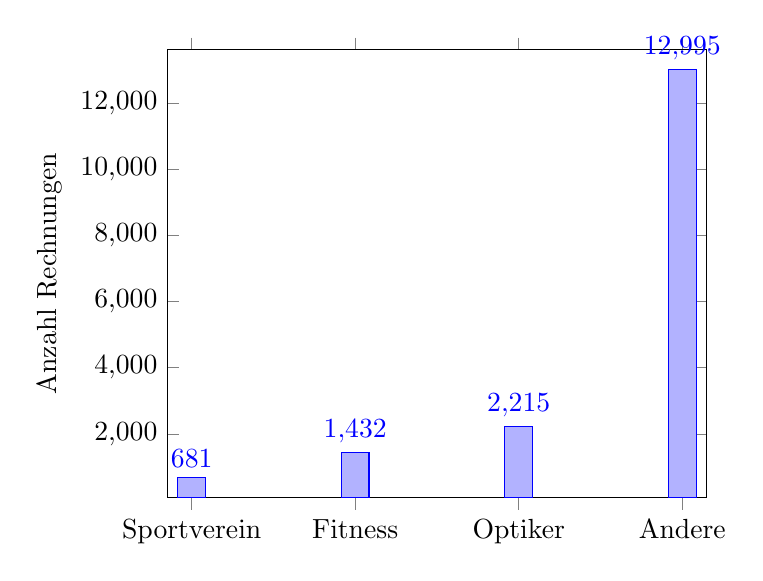
\begin{tikzpicture}
        \begin{axis}[
            ybar,
        	ylabel=Anzahl Rechnungen,
        	enlargelimits=0.05,
            symbolic x coords={Sportverein,Fitness,Optiker,Andere},
            y tick label style={/pgf/number format/fixed},
            scaled y ticks=false,
            xtick=data,
            nodes near coords,
            nodes near coords align={vertical},
        ]
            \addplot 
        	    coordinates {(Sportverein, 681) (Fitness, 1432) (Optiker, 2215) (Andere, 12995)};
        \end{axis}
    \end{tikzpicture}
\end{figure}

\subsubsection{Bild-basierte Rechnungsklassifizierung}

% http://citeseerx.ist.psu.edu/viewdoc/download?doi=10.1.1.414.9846&rep=rep1&type=pdf

% Analog der Klassifizierung von Objekten auf Fotos, ist es auch denkbar, Rechnung mit Hilfe diesem Bild-basiertem Vorgehen zu klassifizieren.

Auf dem Machine Learning Blog \enquote{Towards Data Science} beschreiben und vergleichen diverse Autoren verschiedenste Modelle im Bereich der Computer Vision. Der Blog bietet einen guten Überblick über die aktuellen Methoden zur Klassifizierung von Bildern. So werden im Juli 2017 die Residual Networks (kurz ResNet), entwickelt von \textcite{He2015}, als die bahnbrechendse Eingabe beim ImageNet LSVRC Wettbewerb\footnote{Die ImageNet Large Scale Visiual Recognition Competition (LSVRC) ist ein Wettbewerb der ImageNet Organisation, bei welcher hunderte Data Scientists ihre Modelle im Bereich der Computer Vision vergleichen. TODO: Quelle} der letzten Jahre bezeichnet~\autocite{Fungg2017ResNet}. Im September 2018 beschreibt \textcite{SHTsuang2018Inception} das InceptionV4 Netzwerk von Google, welches vom GoogLeNet abgeleitet und mit den Ideen aus dem ResNet erweitert wurde. Das Modell erzielt noch bessere Resultate als das ResNet selbst. Im gleichen Artikel wird auch das Inception-ResNet-V2 vorgestellt, welches im Vergleich zum InceptionV4 Netzwerk schneller trainiert werden kann und zugleich etwas bessere Resultate erzielt. 

In einem Blog Post auf dem Google AI Blog präsentieren Forscher aus dem Google Brain Team das NASNet. NASNet ist ein Modell zur Klassifizierung von Bildern, welches durch die Anwendung von Machine Learning designed wurde~\autocite{GoogleNasNet}. Unter dem Codename AutoML publiziert das Google Brain Team einen Ansatz, bei welchem ein Neuronales Netzwerk ein anderes erstellt - eine künstliche Intelligenz, welche eine neue künstliche Intelligenz schafft. Mit diesem Ansatz kann das sehr aufwendige Design eines Neuronalen Netzwerks vereinfacht beziehungsweise automatisiert werden~\autocite{GoogleAutoML}.

\begin{wrapfigure}{r}{0.6\textwidth} 
    \caption{Vergleich des vom Google Brain Team präsentierten NASNet mit bestehenden Netzwerken zur Klassifizierung von Bildern des ImageNet Datensatzes. Es wird die Treffergenauigkeit, der Prozentsatz richtig Klassifizierter Bilder der Gesamtheit aller Bilder, der Anzahl benötigter Operationen, sprich die Komplexität des Netzwerks, gegenübergestellt.}
    \label{nasnet-comparision}
    \centering
    \includegraphics[width=0.55\textwidth]{graphics/nasnet-comparision.jpg}
    \caption*{Quelle: \textcite{GoogleNasNet}}
\end{wrapfigure}
Als Teil des selben Blog Posts, in welchem das NASNet präsentiert wird, vergleichen die Forscher von Google das Modell mit anderen Netzwerken, wie dem ResNet und dem Inception-ResNet-V2. Der Abbildung \ref{nasnet-comparision} ist zu entnehmen, dass das vom Google Brain Team präsentierte NASNet, in der \enquote{medium} Ausprägung, trotz reduzierter Anzahl an benötigter Operationen, sprich reduzierter Komplexität, eine verbesserte Treffergenauigkeit als die bisherigen Netzwerke erzielt. In der \enquote{large} Ausprägung kann das NASNet durch eine erhöhte Komplexität eine noch bessere Treffergenauigkeit erzielen~\autocite{GoogleNasNet}.

% ResNet Arxiv: https://arxiv.org/abs/1512.03385
% ResNet: https://towardsdatascience.com/an-overview-of-resnet-and-its-variants-5281e2f56035
% DRM Arxiv: https://arxiv.org/abs/1512.03385
% DRN: https://towardsdatascience.com/review-drn-dilated-residual-networks-image-classification-semantic-segmentation-d527e1a8fb5
% InceptionV4: https://towardsdatascience.com/review-inception-v4-evolved-from-googlenet-merged-with-resnet-idea-image-classification-5e8c339d18bc

% NASNet: https://ai.googleblog.com/2017/11/automl-for-large-scale-image.html

% NASNet example https://www.tensorflow.org/hub/tutorials/image_retraining

% AutoML: https://ai.googleblog.com/2017/05/using-machine-learning-to-explore.html


% TODO: Dilated Residual Network beschreiben: Veränderung der Convolutions in einem ResNet zu einem Grid anstelle der herkömmlichen convolution.

Im folgenden wird das ResNet, das Inception-ResNet-V2 sowie das NASNet large Netzwerk angewendet, um die bisher bei der AXA eingereichten Rechnung zu klassifizieren.

Um Bilderkennungsmodelle mit Millionen von Parametern zu trainieren, werden viele Trainingsdaten und eine enorme Kapazität an Rechenleistung benötigt. Das Konzept des Transfer Learning bietet eine Möglichkeit, diese beiden Problematiken zu Umgehen und dabei nur wenig Treffergenauigkeit einzubüssen. Beim Transfer Learning wird ein Modell mit Hilfe eines Datensatzes trainiert, welcher nichts mit der eigentlichen Problemstellung zu tun hat. Das trainierte Modell wird dann mit den für die Problemstellung relevanten Daten weiter trainiert. Dies wird als Fine Tuning bezeichnet~\autocite{TensorflowImageRetraining, TDSTransferLearning}.

Um die Rechnungen zu klassifizieren wird Transfer Learning angewendet, indem die genannten Modelle auf dem ImageNet Datensatz trainiert werden, bevor die eigentliche Problemstellung angegangen wird.

Nach dem Training auf dem ImageNet Datensatz werden die letzten Schichten des Netzwerks, jene die für die Klassifizierung zuständig sind, durch ein neues Klassifizierungsnetzwerk ersetzt. Dadurch wird der Trainingseffekt durch den ImageNet Datensatz beibehalten und die Klassifizierung so angepasst, dass sie die Einteilung in die vier vorliegenden Klassen erlaubt.

Das Klassifizierungsnetzwerk (vgl. Abbildung \ref{image-classification-model}), welches zur Anwendung kommt, besteht aus einem Convolution Layer sowie drei Fully Connected Layer. Zwischen den Fully Connected Layern sind zwei Dropout Layer zur Reduzierung des Overfitting eingeschoben.

% \begin{wrapfigure}{L}{0.4\textwidth} 
\begin{figure}[h]
    \caption{Neuronales Netzwerk, welches bei der Text-basierten Klassifizierung zur Anwendung kommt. Der Input aus dem Wörterbuch wird durch zwei Fully Connected und einem Dropout Layer in einen One Hot Encoded Output transformiert, der die erkannte Klasse repräsentiert.}
    \label{image-classification-model}
    \centering
    \includegraphics[width=0.2\textwidth]{graphics/image-classification-results/model.pdf}
%\end{wrapfigure}
\end{figure}

Die genannten Modelle werden mit 80\% der vorhandenen Daten trainiert, die übrigen 20\% werden benötigt, um den Trainingsfortschritt zu prüfen. Mit diesen 20\% Testdaten soll ein allfälliges Overfitting erkannt werden.

Die Abbildung \ref{image-class-results} zeigt das Training der genannten Modelle während 60 Trainingsepochen (Trainingseinheiten). \ref{image-class-results:a} und \ref{image-class-results:b} zeigen die Treffergenauigkeit respektive das loss während dem Training. Während dem Training steigt die Treffergenauigkeit stetig an und das loss sinkt stetig. Dies zeigt, dass die gewählten Modelle lernen. \ref{image-class-results:c} und \ref{image-class-results:d} zeigen die Treffergenauigkeit respektive das loss bei der Anwendung des Modells auf den Testdaten. 

Die einzelnen Modelle zeigen eine Treffergenauigkeit von TODO\% (ResNet, Epoche TODO), TODO\% (Inception-ResNet-V2, Epoche TODO) beziehungsweise TODO\% (NASNet, Epoche TODO).

Das auf dem TODO TODO TODO\todo{TODO} basierende Modell hat mit einer Treffergenauigkeit von \todo{TODO}\% nach \todo{TODO} Epochen die höchste Treffergenauigkeit auf den Testdaten. 

Neben der auch nach 60 Epochen noch leicht steigenden Treffergenauigkeit hat das loss auf den Testdaten (vgl. Abbildung \ref{image-class-results:d}) bereits nach 25 Epochen den Wendepunkt erreicht. Dies ist ein Indikator dafür, dass das Modell beginnt Auswendig zu lernen.

\begin{figure}[ht] 
  \captionsetup{width=.8\linewidth}
  \caption{Statistiken aus dem Training der Bild-basierten Klassifizierung von Rechnungen mit den ResNet, Inception-ResNetV2 und NASNet Netzwerken.}
  \label{image-class-results} 
  \includegraphics[width=0.5\textwidth]{graphics/image-classification-results/legend.pdf}
  \begin{subfigure}[b]{0.5\linewidth}
    \centering
    \includegraphics[width=0.75\linewidth]{graphics/image-classification-results/acc.pdf} 
    \caption{Treffergenauigkeit} 
    \label{image-class-results:a} 
    \vspace{2ex}
  \end{subfigure}%% 
  \begin{subfigure}[b]{0.5\linewidth}
    \centering
    \includegraphics[width=0.75\linewidth]{graphics/image-classification-results/loss.pdf} 
    \caption{loss} 
    \label{image-class-results:b} 
    \vspace{2ex}
  \end{subfigure} 
  \begin{subfigure}[b]{0.5\linewidth}
    \centering
    \includegraphics[width=0.75\linewidth]{graphics/image-classification-results/val_acc.pdf} 
    \caption{Treffergenauigkeit bei den Testdaten} 
    \label{image-class-results:c} 
  \end{subfigure}%%
  \begin{subfigure}[b]{0.5\linewidth}
    \centering
    \includegraphics[width=0.75\linewidth]{graphics/image-classification-results/val_loss.pdf} 
    \caption{loss bei den Testdaten} 
    \label{image-class-results:d} 
  \end{subfigure}
  \centering
\end{figure}

\todo[inline]{Update graphics \& legend with NASNet Results, also revisti the paragraph above, whether it holds true for NASNet}

\todo[inline]{Dropout beschreiben, Wahl dieses Modells begründen}


Optimierungspotential:

- https://towardsdatascience.com/deep-learning-performance-cheat-sheet-21374b9c4f45

\textbf{Data augmentation}

https://medium.com/nanonets/how-to-use-deep-learning-when-you-have-limited-data-part-2-data-augmentation-c26971dc8ced


\textbf{Local mimimum through Adam optimizer}

https://towardsdatascience.com/estimating-optimal-learning-rate-for-a-deep-neural-network-ce32f2556ce0


\textbf{Experiment with batch size and number of epochs}

\textbf{Generate Network using AI (or just the optimizer)}

ENAS: https://github.com/carpedm20/ENAS-pytorch
Neural Architecture Search with Reinforcement Learning: https://arxiv.org/abs/1611.01578
Neural Optimizer Search with Reinforcement Learning: https://arxiv.org/abs/1709.07417

\textbf{Weight penalty L1 and L2}

Improve performance and reduce overfitting -> Keeps weights in NN small
-> Have a look at the trained model, are there huge weights? If so, highlight this as a problem




\subsubsection{Text-basierte Rechnungsklassifizierung}
\label{chap:text-based-classification}

\todo[inline]{- Look at the Vocabulary that is created

- Remove diacritics in pre-processing

- Rerun Tesseract

- Rerun classifiers (image and text) without cache

- Als empfehlung in der Thesis: 

-- Stemming um wörter zu generalisieren

-- Teilwörter splitten (Fitness -> Fitness|park -> Fitness|abo)}

Werden die Rechnungen nicht als Bilder angesehen, sondern wird der auf Ihnen aufgedruckte Text als zentraler Aspekt angesehen, so liegt die Klassifizierung der Rechnung aufgrund dieses Textes nahe. Um die Rechnungen allerdings aufgrund des Textes zu Klassifizieren, muss dieser zuerst aus den Bildern der Rechnungen extrahiert werden. Mit Hilfe von Tesseract OCR wird der Text aus den Bildern extrahiert.

Nach dem Extrahieren des Textes aus den Rechnungen wird als erstes ein Wörterbuch gebildet, welches das Word embedding ermöglicht. Das Word embedding dieses Wörterbuchs ist sehr einfach gehalten und erlaubt keine Rückschlüsse auf die Bedeutung der Wörter aufgrund des resultierenden Vektors.

Das Wörterbuch wird erstellt, indem der Text erst in Kleinbuchstaben umgewandelt und anschliessend bei Leerzeichen getrennt wird. Es werden alle Stopp-Wörter wie \enquote{und}, \enquote{ein} und \enquote{diese} entfernt, da aus ihnen keine Informationen gewonnen werden können. Es werden die häufigsten Wörter ermittelt, zu welchen sich das Wörterbuch je eine eindeutige Zahl merkt. Diese Zahl dient als Abbildung des jeweiligen Wortes. Das Wörterbuch hält sich nur die häufigsten Wörter um die Komplexität gering zu halten.

Nach dem Wörterbuch wird ein Klassifizierungsmodell erstellt. Input dieses Netzwerks ist ein Vektor in der Länge der Anzahl Wörter im Wörterbuch. Pro Wort wird in diesem Vektor die Präsenz beziehungsweise Absenz des Wortes innerhalb einer Rechnung angegeben. Nach dem Input folgen ein Fully Connected Layer. Dieser ist durch einen Dropout Layer mit dem Fully Connected Output Layer verbunden (vgl. Abbildung \ref{text-classification-model}). 

% \begin{wrapfigure}{r}{0.4\textwidth} 
\begin{figure}[h]
    \caption{Neuronales Netzwerk, welches bei der Text-basierten Klassifizierung zur Anwendung kommt. Der Input aus dem Wörterbuch wird durch zwei Fully Connected und einem Dropout Layer in einen One Hot Encoded Output transformiert, der die erkannte Klasse repräsentiert.}
    \label{text-classification-model}
    \centering
    \includegraphics[width=0.2\textwidth]{graphics/text-classification/model.pdf}
% \end{wrapfigure}
\end{figure}

\todo[inline]{- Input layer bei diesen Grafiken ergänzen

- Breite der Layer in der Grafik ergänzen}


TODO



Bei der Text-basierten Klassifizierung erreicht das loss auf den Testdaten nach 23 Epochen den Wendepunkt (vgl Abbildung \ref{text-class-results:val_loss}). Dabei wird eine Treffergenauigkeit von 98.4\% erreicht (vgl. Abbildung \ref{text-class-results:val_acc}). Die Treffergenauigkeit liegt bei diesem Ansatz somit deutlich höher als beim Bild-basierten Ansatz.

\begin{figure}[ht] 
  \captionsetup{width=.8\linewidth}
  \caption{Statistiken aus dem Training der Text-basierten Klassifizierung von Rechnungen.}
  \label{image-class-results}
  \begin{subfigure}[b]{0.5\linewidth}
    \centering
    \includegraphics[width=0.75\linewidth]{graphics/text-classification/acc.pdf} 
    \caption{Treffergenauigkeit} 
    \label{text-class-results:val} 
    \vspace{2ex}
  \end{subfigure}%% 
  \begin{subfigure}[b]{0.5\linewidth}
    \centering
    \includegraphics[width=0.75\linewidth]{graphics/text-classification/loss.pdf} 
    \caption{loss} 
    \label{text-class-results:loss} 
    \vspace{2ex}
  \end{subfigure} 
  \begin{subfigure}[b]{0.5\linewidth}
    \centering
    \includegraphics[width=0.75\linewidth]{graphics/text-classification/val_acc.pdf} 
    \caption{Treffergenauigkeit bei den Testdaten} 
    \label{text-class-results:val_acc} 
  \end{subfigure}%%
  \begin{subfigure}[b]{0.5\linewidth}
    \centering
    \includegraphics[width=0.75\linewidth]{graphics/text-classification/val_loss.pdf} 
    \caption{loss bei den Testdaten} 
    \label{text-class-results:val_loss} 
  \end{subfigure}
  \centering
\end{figure}

Die falsche Klassifizierung einer Rechnung ist vor allem dann problematisch, wenn diese einer Klasse zugewiesen wird, welche automatisch Verarbeitet wird. Die Confusion Matrix in Abbildung \ref{text-classification-cm} zeigt, dass das Text-basierte Modell aus 3367 Testdatensätzen sechs Rechnungen fälschlicherweise als Fitness Rechnungen und fünf Rechnungen fälschlicherweise als Rechnungen für einen Sportverein klassifiziert hat. Dies ergibt eine Genauigkeit|Sensitivität von xx\% (Fitness), xx\% (Optiker) respektive xx\5 (Sportverein). 

\todo[inline]{Precision und Recall anhand der Confusion Matrix besprechen. Error analysis, wie dies im Buch Machine Learning Yearning beschrieben ist beschreiben. Daraus die Fehler/das Potential, welche unten folgend, ableiten und ergänzen.}

\begin{wrapfigure}{r}{0.5\textwidth} 
    \caption{Confusion Matrix nach 23 Epochen Training des Text-basierten Modells. Das Modell klassifiziert sechs Rechnungen fälschlicherweise als Fitness Rechnung und fünf Rechnungen fälschlicherweise als Rechnungen für einen Sportverein.}
    \label{text-classification-cm}
    \centering
    \includegraphics[width=0.5\textwidth]{graphics/text-classification/cm_22.png}
\end{wrapfigure}

Die Insgesamt 53 falsch klassifizierten Rechnungen aus dem Testdatensatz wurden zusammen mit den während dem Training falsch klassifizierten Rechnungen einer Fehleranalyse unterzogen. Während dieser Analyse wurden folgende Probleme identifiziert \todo{Reference the Machine Learning Yearning book that describes this approach}

Ein Problem, welches sofort ins Auge sticht, sind die Ergebnisse des Optical Character Recognition Systems. Diese sind teilweise sehr dürftig. Durch die mässige Qualität fotografierter Rechnungen können gewisse Wörter nur schlecht oder garnicht erkannt werden. Besonders eine schlechte Ausleuchtung scheint Tesseract OCR Mühe zu bereiten.

Durch die ungenauigkeiten während dem OCR Prozess entstehen viele Wörter mit Schreibfehlern. Das Wörterbuch erkennt aber nur Wörter, welche mit den gelernten Wörtern identisch sind. Wurde während dem Training des Wörterbuchs ein Wort nie in einer gewissen falschen Schreibweise angetroffen, so ist es für das Klassifizierungsmodell nutzlos.

\subsubsection{Schlussfolgerungen}

\todo[inline]{- Text-basiertes Modell performt sehr gut

- Trotzdem noch einige Verbesserungsptentiale

- Einbau einer Probability Schwelle um falsch-Klassifizierungen zu vermeiden

- folgende Potential beschreiben:}

\textbf{OCR Fehler}

Um die Resultate dieses Zwischenschritts zu verbesseren, sieht der Autor folgende Optionen.

\begin{itemize}
    \item Es könnte versucht werden, dass LSTM Modell, welches dem Tesseract OCR System zugrunde liegt, auf die Rechnungen zu trainieren. Das OCR System kann durch Training mit Schriftzügen und Buchstaben, auf welche das System bisher nicht Trainiert wurde, einiges an Treffergenauigkeit gewinnen. Das System sollte aus diesem Grund auf die gängigsten Schriften der Rechnungen trainiert werden\~{TesseractTraining}.
    \item Aktuell wurde das OCR System mit den Sprachen Deutsch, Englisch, Französisch und Italienisch instruiert. Nach dem ersten Lauf mit diesen vier Sprachen könnte versucht werden, mit einem KI-Modell die Sprache zu erkennen. Anschliessen könnte das OCR System mit nur dieser Sprache erneut verwendet werden. Somit könnten beispielsweise falsche diakritische Zeichen durch eine Körnung des Bildes vermindert werden. Auch erlaubt dieses Vorgehen dem OCR System die verbesserte Erkennung durch dem System bekannte Wörter.
    \item Die Ergebnisse aus dem OCR Schritt könnten durch ein Rechtschreibe- und Grammatikkorrektur-Modell verbessert werden. \todo{Referenz auf Einleitungskapitel}
\end{itemize}

\textbf{Verbessertes WordEmbedding}

Anstelle des aktuell verwendeten, einfachen Word Tokenizer könnte ein komplexeres WordEmbedding\todo{Referenz auf Einleitungskapitel} angewendet werden. Jüngste Forschungen zeigen, dass auch in diesem Bereich dank Transfer Learning gute Ergebnisse erzielt werden können. Beispielsweise wurde im Oktober 2018 mit BERT\footnote{Bidirectional Encoder Representations from Transformers, kurz BERT, ist ein Modell zur repräsentation von natürlicher Sprache. Das Modell des Google Reasearch Team bricht viele bisherige Rekorde bei Natural Language Processing Wettbewerben~\autocite{Devlin2018}} ein sehr erfolgreiches Modell im Bereich des Natural Language Processing publiziert, welches als Grundlage für das Transfer Learning dienen kann~\autocite{Devlin2018}.

\todo[inline]{
Klassifizierung von Rechnungen

Evtl. verschiedene Ansätze

- OCR -> (SpellCorrection ->) WordEmbedding -> classification

- Pixel -> classification

- OCR -> (SpellCorrection ->) InformationExtraction -> classification

Bewertung der Ergebnisse
}

\todo[inline]{Dropout und dilating beschreiben}

\subsection{Teil 2 - Informationsextraktion}

% Massive comparision of object detection models: https://medium.com/@jonathan_hui/object-detection-speed-and-accuracy-comparison-faster-r-cnn-r-fcn-ssd-and-yolo-5425656ae359
% Do these results hold true for our "special" case of papaer region detection?

% https://rectlabel.com

\subsection{Ausblick}

Mägliches Potential

Rotations-Erkennung (Verbessert evtl. OCR, etc., see 5a6af27e0cf2ab51c3ec3c70.pdf.png for OCR result)

Filter out training data of low quality images...

Kontrast extrem wichtig für OCR, mehr als Körnung und Schärfe....

Rotation hat bei OCR klassifizierung einen starken einfluss...

Extrem viele QualiCert Belege, diese aber oft handschriftlich, IE ist wohl schwer



Fehler in den Trainingsdaten. Error analysis war wichtig. Zitiere dabei das Buch dazu. Finde mit einem diff die ursprünglich falsch klassifizierten und quantifiziere dies


Blacklisting von Wörtern wie "Einzahlungsschein" da dies als Sportclub klassifiziert wird -.-" -> Alle wörter die nicht mehr als n levenstein distance haben blacklistenmmacjp